\documentclass[8pt, a4paper, oneside, twocolumn]{extarticle}
\usepackage{graphicx}
\usepackage[export]{adjustbox}
\usepackage[compact]{titlesec}  % documentation: http://mirror.iopb.res.in/tex-archive/macros/latex/contrib/titlesec/titlesec.pdf  
\usepackage{kotex}
\usepackage[left=0.8cm, right=0.8cm, top=2cm, bottom=0.3cm, a4paper]{geometry}
\usepackage{amsmath}
\usepackage{ulem}
\usepackage{amssymb}
\usepackage{minted}  % syntax highlighting
\usepackage{enumitem}
\setlist{nolistsep}
\usepackage{fancyhdr} % documentation: http://ctan.math.utah.edu/ctan/tex-archive/macros/latex/contrib/fancyhdr/fancyhdr.pdf
\usepackage{lastpage}  % just so that we can use \pageref {LastPage}
\usepackage{color, hyperref}
% The lines in the table of contents become links to the corresponding pages in the document by simply adding in the preamble of the document the line
\usepackage{tikz}
\usetikzlibrary{positioning,chains,fit,shapes,calc}
\newcommand{\bck}{
    \textbackslash
}
\newcommand{\iph}[2]{
    \includegraphics[width=#1\textwidth,height=#1\textheight,keepaspectratio]{#2}
}
\newcommand{\ph}[1]{
    \includegraphics[width=0.5\textwidth,height=0.5\textheight,keepaspectratio]{#1}
}
\newcommand{\ita}[1]{
    \textit{#1}
}
\newcommand{\swastik}[1]{%
    \begin{tikzpicture}[#1]
        \draw (-1,1)  -- (-1,0) -- (1,0) -- (1,-1);
        \draw (-1,-1) -- (0,-1) -- (0,1) -- (1,1);
    \end{tikzpicture}%
}
\titlespacing*{\section}
{0pt}{0px plus 1px minus 0px}{-2px plus 0px minus 0px}
\titlespacing*{\subsection}
{0pt}{0px plus 1px minus 0px}{0px plus 3px minus 3px}
\titlespacing*{\subsubsection}
{0pt}{0px plus 1px minus 0px}{0px plus 3px minus 3px}
\setlength{\columnseprule}{0.4pt}
\DeclareRobustCommand{\stirling}{\genfrac\{\}{0pt}{}}
\setlength{\parindent}{0pt}  % so that there is no indent of paras.
\setminted{breaklines=true, tabsize=2, breaksymbolleft=}
\begin{document}
\title{\swastik {scale = 0.2} {}Compiler Short Revision Notes{} \swastik {scale = 0.2}}
\author{Sourabh Aggarwal}
\date{Compiled on \today}
\maketitle
\pagenumbering{roman}
\tableofcontents
\newpage
\thispagestyle{fancy}  % else it was not giving fancy header to the first page
\pagenumbering{arabic}
\section{Intro And ML Lex}

$(a \odot b) \vert \epsilon$ represents the language \{"", "ab"\}. 
In writing regular expressions, we will sometimes omit the concatenation 
symbol or the epsilon, and we will assume that Kleene closure "binds tighter" 
than concatenation, and concatenation binds tighter than alternation; so that 
$ab \vert c$ means $(a \odot b) \vert c$, and $(a \vert)$ means $(a \vert \epsilon)$. 
Let us introduce some more abbreviations: [abed] means 
$(a \vert b \vert c \vert 
d)$, [b-g] means [bcdefg], [b-gM-Qkr] means [bcdefgMNOPQkr], M? 
means ($M \vert \epsilon$), and $M^+$ means ($M \odot M^*$). 

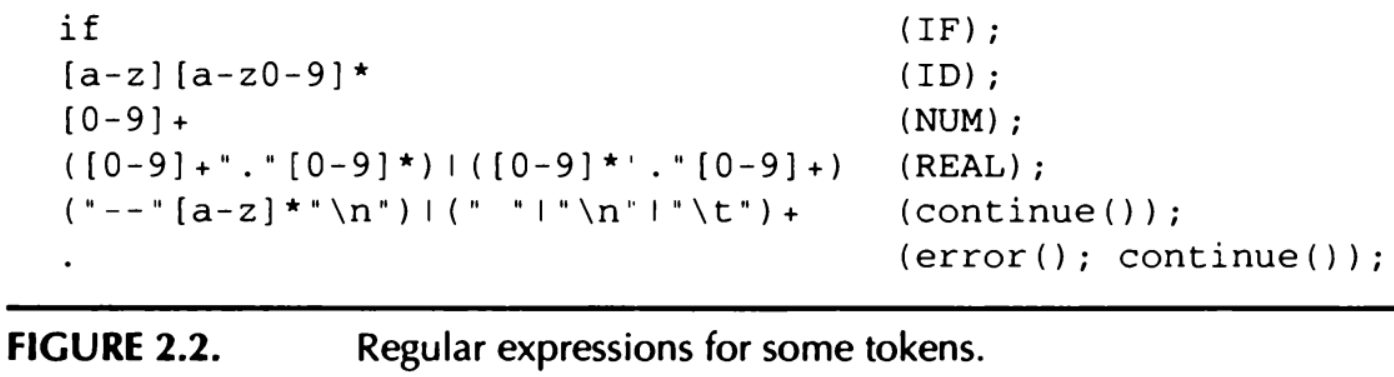
\includegraphics[width=0.5\textwidth,height=0.5\textheight,keepaspectratio]{reg}

Longest match: The longest initial substring of the input that can match any 
regular expression is taken as the next token. 

Rule priority: For a \textbf{particular} longest initial substring, the first regular  
expression that can match determines its token type. This means that the order of 
writing down the regular-expression rules has significance. 

So according to the rules, if8 match as a single 
identifier and not as the two tokens if and 8. And "if 89" begin with a 
reserved word and not by an identifier by rule priority rule. 


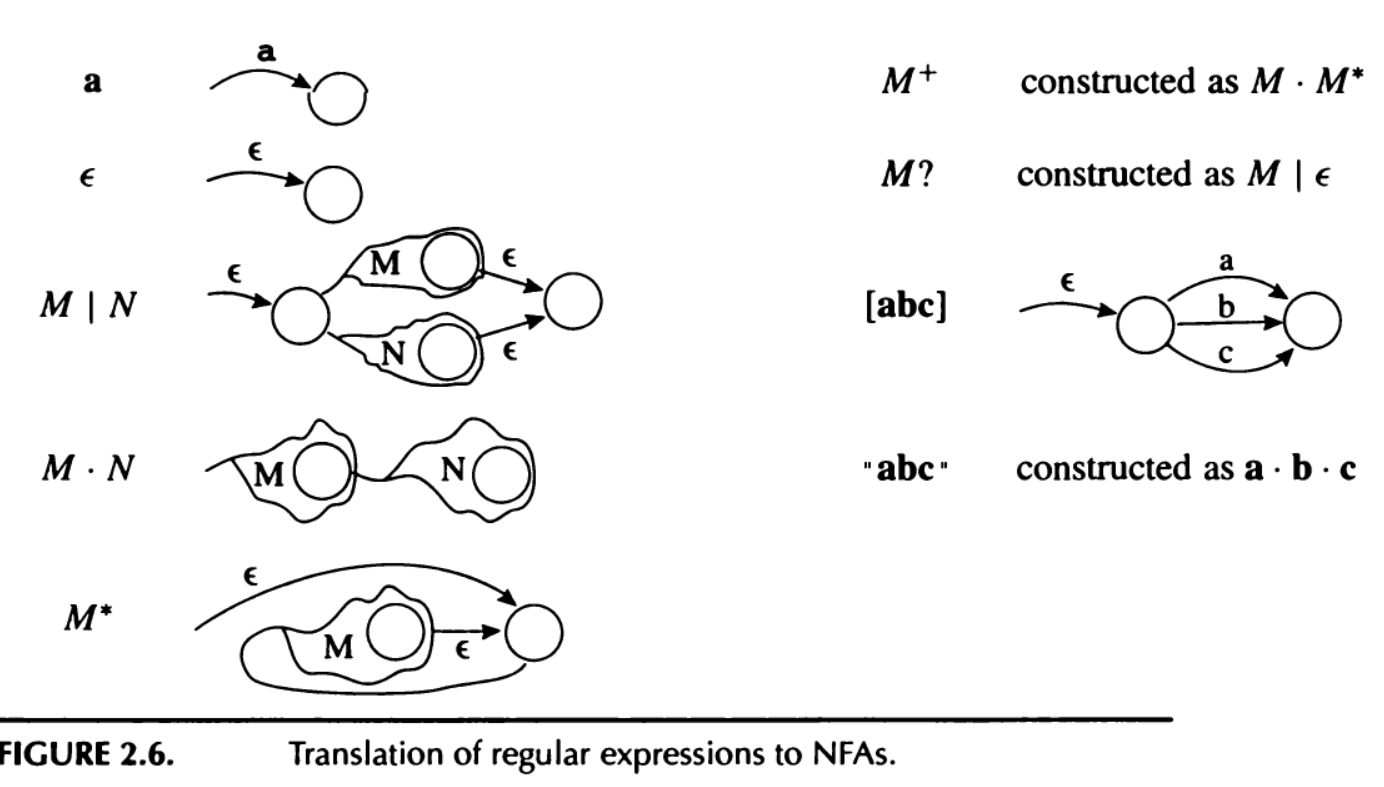
\includegraphics[width=0.5\textwidth,height=0.5\textheight,keepaspectratio]{rtnfa}

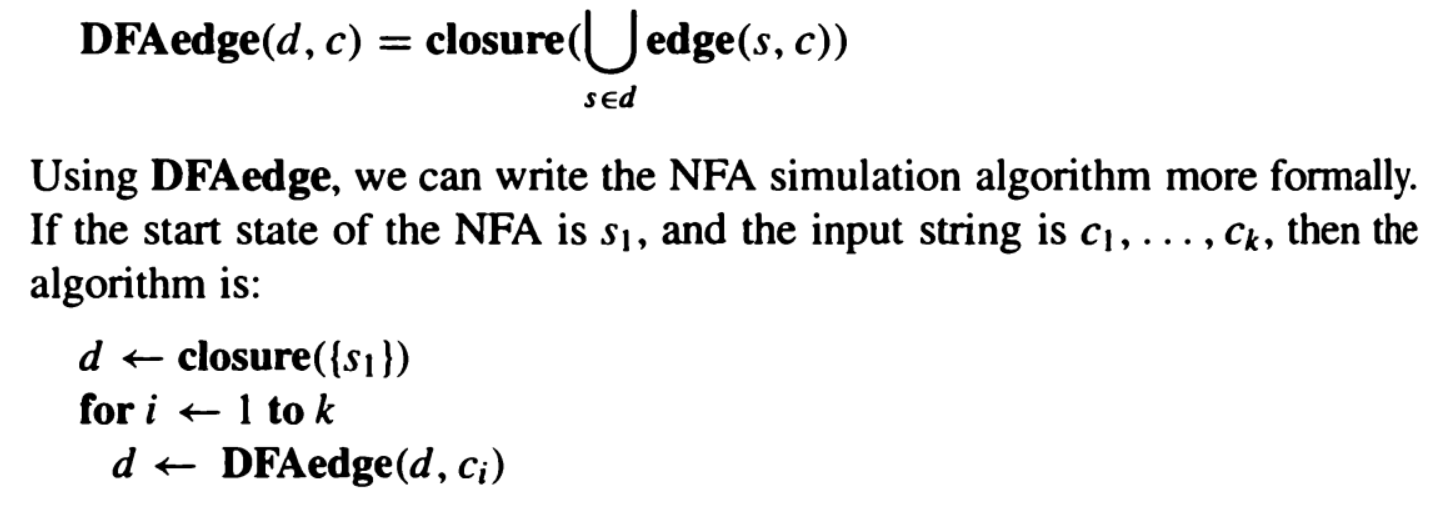
\includegraphics[width=0.5\textwidth,height=0.5\textheight,keepaspectratio]{nfa1}

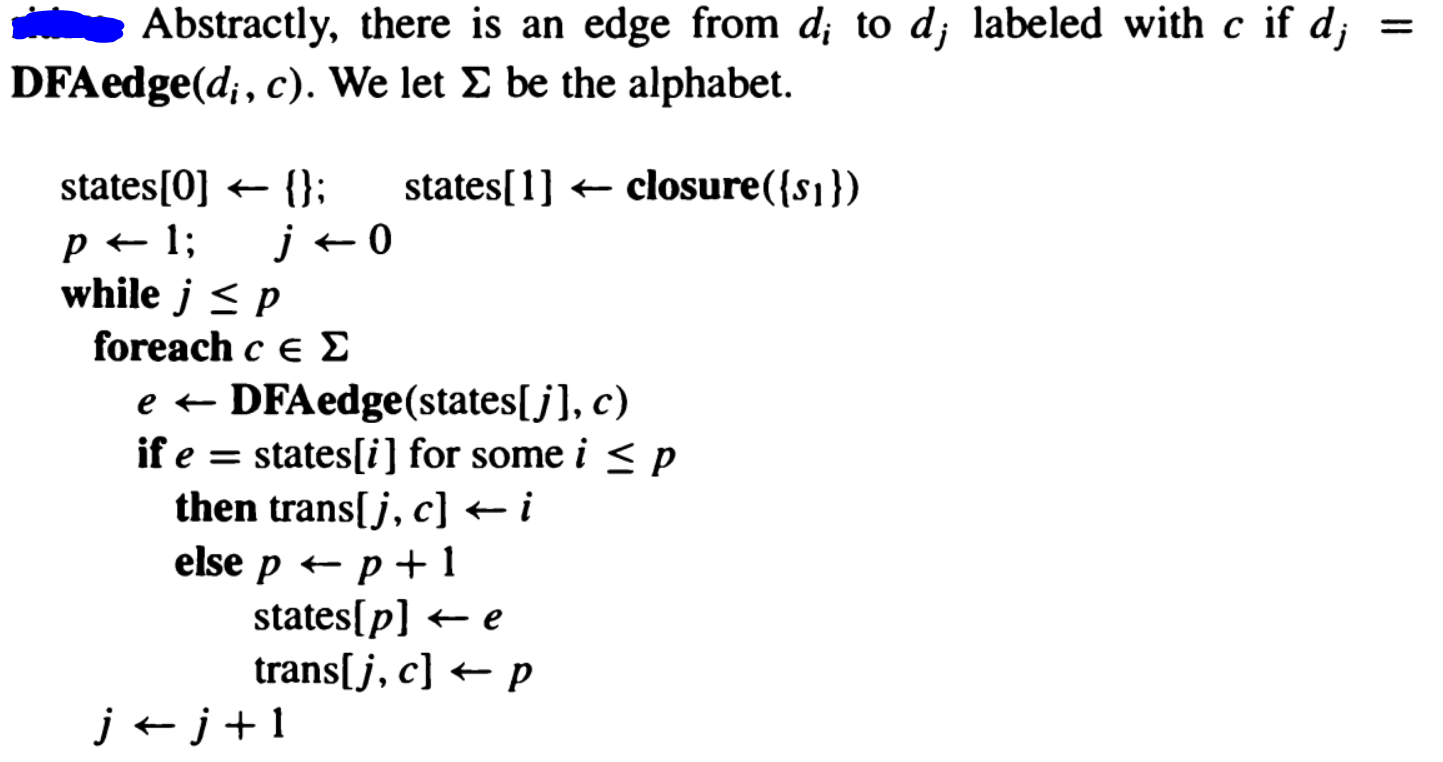
\includegraphics[width=0.5\textwidth,height=0.5\textheight,keepaspectratio]{nfa2}

DFA construction is a mechanical task easily performed by computer, so it 
makes sense to have an automatic lexical analyzer generator to translate  
regular expressions into a DFA. 


The output of ML-Lex is a program in ML - a lexical analyzer that  
interprets a DFA using the algorithm described in Section 2.3 and executes the 
action fragments on each match. The action fragments are just ML statements 
that return token values. 

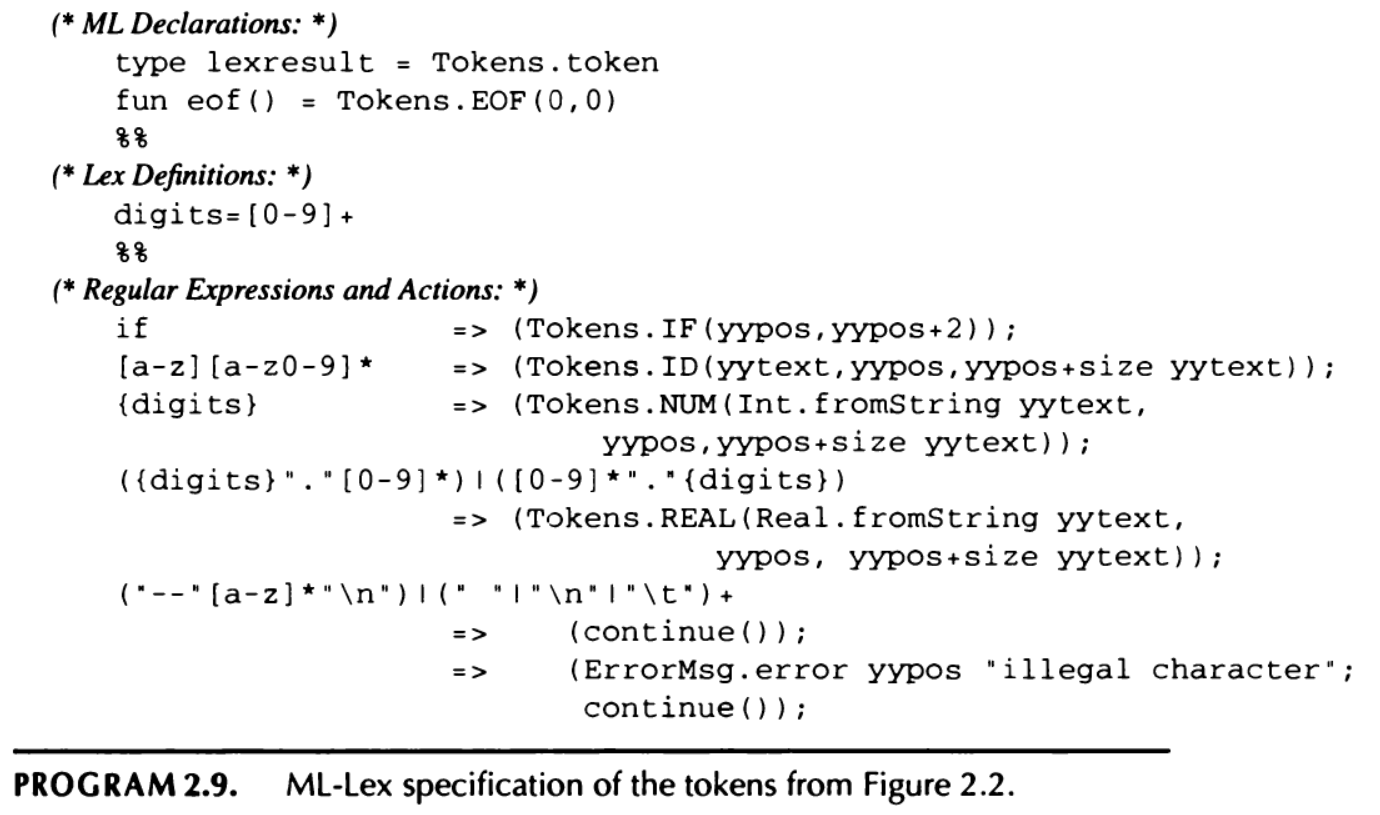
\includegraphics[width=0.5\textwidth,height=0.5\textheight,keepaspectratio]{lex}

The format is: user declarations \%\% ML-Lex definitions \%\% rules

The first part of the specification, above the first \%\% mark, contains  
functions and types written in ML. These must include the type lexresult, 
which is the result type of each call to the lexing function; and the  
function eof, which the lexing engine will call at end of file. This section can 
also contain utility functions for the use of the semantic actions in the third 
section. It is called with the same argument as lex (see \%arg, below), and must return a value of type lexresult. 

The second part of the specification contains regular-expression  
abbreviations and state declarations. For example, the declaration digits=$[0-9]^+$ 
in this section allows the name \{digits\} to stand for a nonempty sequence 
of digits within regular expressions. 

In the definitions section, the user can define named regular expressions, a set of start states, and specify which of the various bells and whistles of ML-Lex are desired.

The third part contains regular expressions and actions. The actions are 
fragments of ordinary ML code. Each action must return a value of type 
lexresult. In this specification, lexresult is a token from the Tokens 
structure. 

In the action fragments, several special variables are available. The string 
matched by the regular expression is yytext. The file position of the  
beginning of the matched string is yypos. The function continue () calls the 
lexical analyzer recursively. 

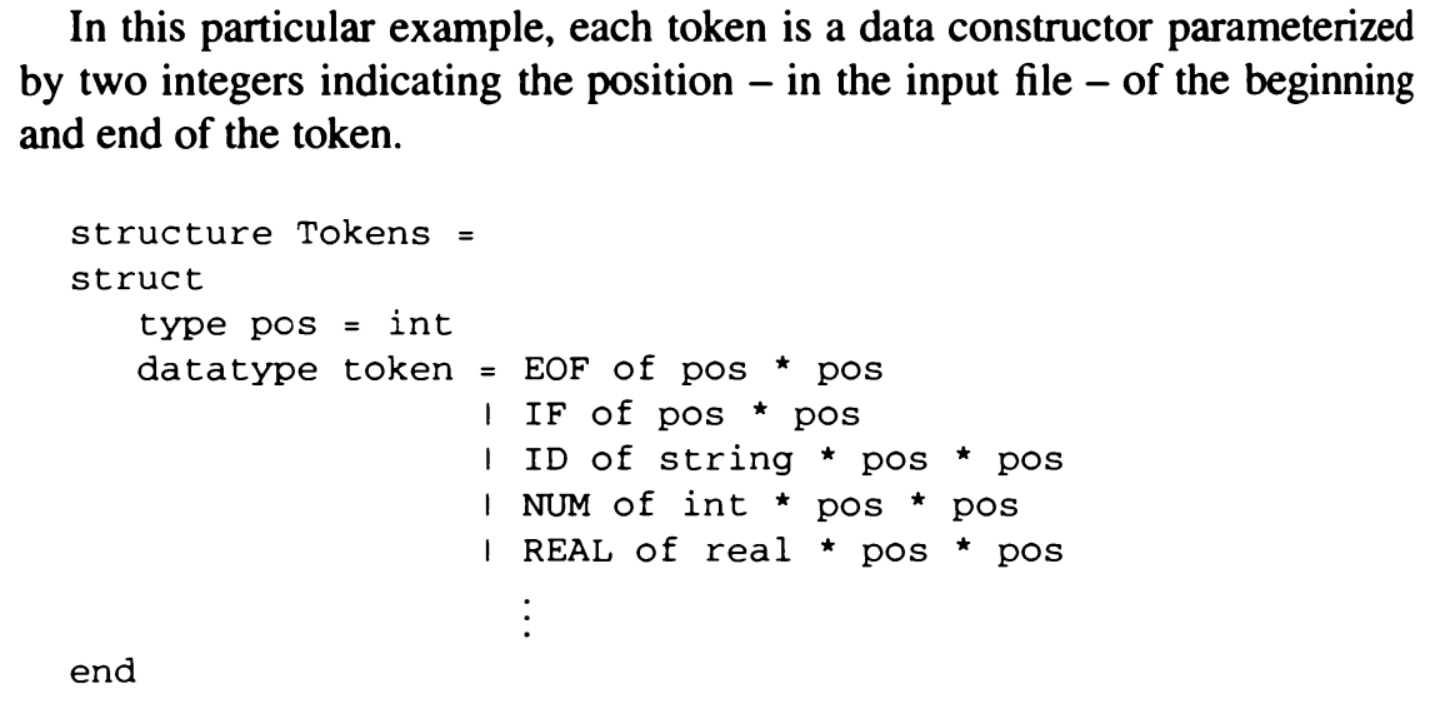
\includegraphics[width=0.5\textwidth,height=0.5\textheight,keepaspectratio]{lex2}

Arguments given to token are called payload.

The tokens are defined by the combined effect of

1. The \%term commands used in the ML-Yacc declaration section of your ML-Yacc
specification. These may add extra values to the token function’s argument and
thus extend the payload.

2. The lexresult type declaration in the user declarations of your ML-Lex specification

If a token has been defined by the \%term command in the .yacc file with no type,
then its payload is usually two integers - its the \%pos declaration which says so, see
chapter 9.4.3 on page 22. For example, looking at the SML/NJ compiler, we see that
the semicolon is defined by the ML-Yacc \%term command in file ml.grm as SEMICOLON.
There is no type specification. The payload is two integers specifying the character
positions in the source file of the start and end of the semicolon:
\begin{minted}{SML}
<INITIAL>";" => (Tokens.SEMICOLON(yypos,yypos+1));
\end{minted}
If a token has been defined in ML-Yacc with a type, then its payload will be a value
of that type, followed by two integers - again, its the \%pos declaration which calls for
those two integers, see chapter 9.4.3 on page 22.. For example, looking at the SML/NJ
compiler, we see that a real number is defined by the ML-Yacc \%term command in file
ml.grm as REAL of string. The payload is therefore a string followed by two integers
specifying the character position in the source file of the start and end of the real number:
\begin{minted}{SML}
<INITIAL>{real} => (Tokens.REAL(yytext,
yypos,
yypos+size yytext));
\end{minted}

But sometimes the step-by-step, state-transition model of automata is  
appropriate. ML-Lex has a mechanism to mix states with regular expressions. 
One can declare a set of start states; each regular expression can be prefixed 
by the set of start states in which it is valid. The action fragments can  
explicitly change the start state. In effect, we have a finite automaton whose edges 
are labeled, not by single symbols, but by regular expressions. This example 
shows a language with simple identifiers, if tokens, and comments delimited 
by (* and *) brackets: 

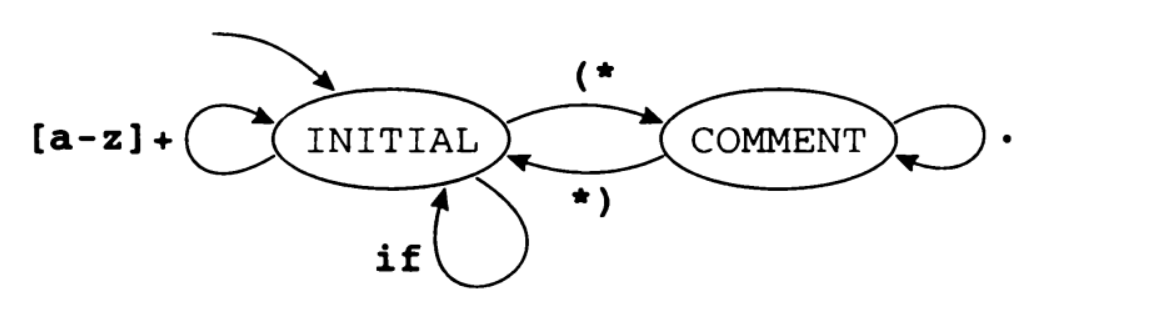
\includegraphics[width=0.5\textwidth,height=0.5\textheight,keepaspectratio]{lex3}

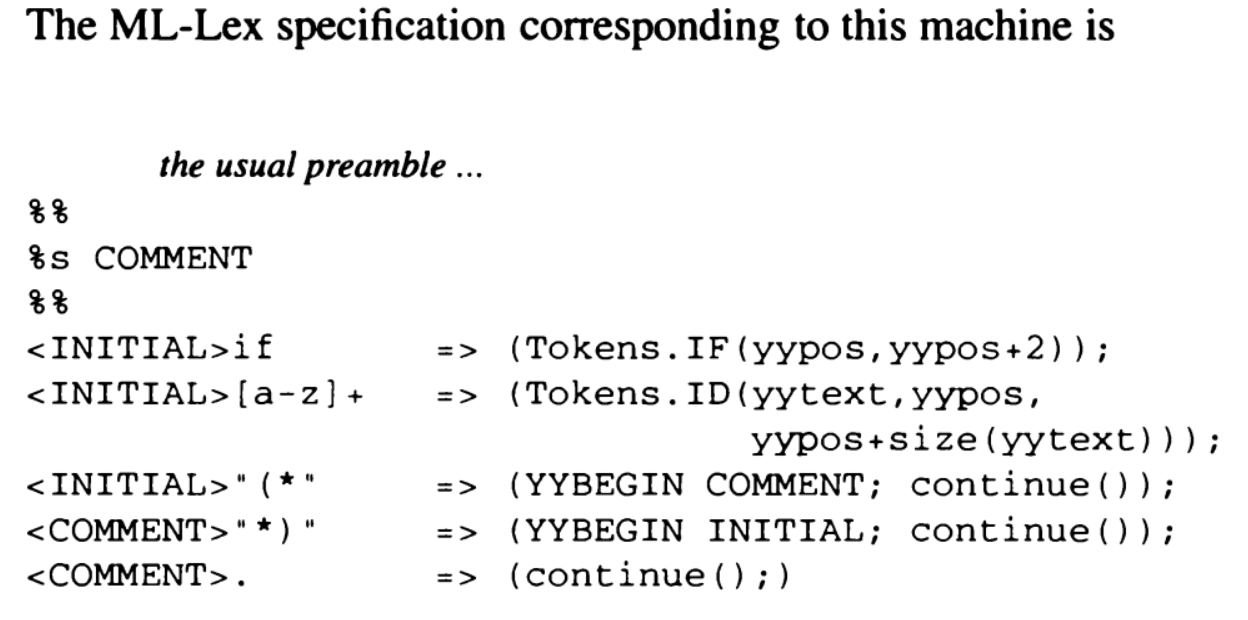
\includegraphics[width=0.5\textwidth,height=0.5\textheight,keepaspectratio]{lex4}

This example can be easily augmented to handle nested comments, via a 
global variable that is incremented and decremented in the semantic actions. 

Any regular expression not prefixed by a $<state>$ operates in all states; this  
feature is rarely useful. 

Certain rules
\begin{itemize}
    \item     An individual character stands for itself, except for the reserved characters 
    \begin{minted}{cpp}
     ? * + | ( ) ^ $ / ; . = < > [ { " \  $

    \end{minted}

    \item A backslash followed by one of the reserved characters stands for that character. 

    \item Inside the brackets, only the symbols \begin{minted}{cpp} 
    \ - ^ 
\end{minted}
 are reserved. An initial up-arrow \^{} stands for the complement of the characters listed, e.g. [\^{}abc] stands any character except a, b, or c.
    \item  To include \^{} literally in a bracketed set, put it anywhere but first; to include - literally in a set, put it first or last. 
    \item The dot . character stands for any character except newline, i.e. the same as \begin{minted}{cpp}
        [^\n]
    \end{minted}
    \item The following special escape sequences are available, inside or outside of square brackets: 
    \begin{minted}{SML}
    \b backspace
    \n newline
    \t horizontal tab
    \ddd where ddd is a 3 digit decimal escape
    \end{minted}
    \item Any regular expression may be enclosed in parentheses ( ) for syntactic (but, as
    usual, not semantic) effect
    \item A sequence of characters will stand for itself (reserved characters will be taken literally) if it is enclosed in double quotes " ".
    \item A postfix repetition range \{a, b\} where a and b are small integers stands for any number of repetitions between a and b of the preceding expression. The notation \{a\} stands for exactly a repetitions. Ex: [0-9]\{3\}
    Any three-digit decimal number. 
    \item The rules should match all possible input. If some input occurs that does not match any rule, the lexer created by ML-Lex will raise an exception LexError.
    \item  The user may recursively call the lexing function with lex(). (If \%arg is used, the lexing function may be re-invoked with the same argument by using continue().) This is convenient for ignoring white space or comments silently:
    \begin{minted}{SML}
    [\ \t\n]+       => ( lex());
    \end{minted}
    \item To switch start states, the user may call YYBEGIN with the name of a start state. 
    \item If the lexer is to be used with the ML-Yacc parser, then additional glue declarations
    are needed:
    \begin{minted}{SML}
    5 structure T = Tokens
    6 type pos = int (* Position in file *)
    7 type svalue = T.svalue
    8 type (’a,’b) token = (’a,’b) T.token
    9 type lexresult = (svalue,pos) token
    10 type lexarg = string
    11 type arg = lexarg
    12 val linep = ref 1; (* Line pointer *)
    \end{minted}
    Lines 5 through 9 provide the basic glue. On line 9, lexresult returns the type of the
result returned by the rule actions.
If you are passing a parameter to the lexer, then you also need the additional glue
in lines 10 through 11. The lexer offers the possibility of counting lines using value yylineno described in
chapter 7.3.6. If you prefer to do this yourself with variable linep, you will need the
declaration on line 12
    \item Running ML - Lex file: From the Unix shell, run \begin{minted}{SML} 
        sml-lex myfile.lex 
        The output file will be myfile.lex.sml. The extension .lex is not required but is recommended. 
    \end{minted}
\end{itemize}

To get messages for lexer errors and unwelcome characters (note: l1 is the lineno. and l2 is the position in that line):
\begin{minted}{SML}
val error : string * int * int -> unit = fn
(e,l1,l2) => TextIO.output(TextIO.stdOut,"lex:line "
^Int.toString l1^" l2="^Int.toString l2
^": "^e^"\n")
val badCh : string * string * int * int -> unit = fn
(fileName,bad,line,col) =>
TextIO.output(TextIO.stdOut,fileName^"["
^Int.toString line^"."^Int.toString col
^"] Invalid character \""^bad^"\"\n");
\end{minted}

A typical error is to
forget to close an ongoing comment. If you allow ML style nested comments (* ... (*
... *) ... *) then you will need some management of nested comments and possible
end-of-file errors in the lexer. 
\begin{minted}{SML}
    21 val mlCommentStack : (string*int) list ref = ref [];
    22 val eof = fn fileName =>
    23 (if (!mlCommentStack)=[] then ()
    24 else let val (file,line) = hd (!mlCommentStack)
    25 in TextIO.output(TextIO.stdOut,
    26 " I am surprized to find the
    27 ^" end of file \""fileName^"\"\n"
    28 ^" in a block comment which began"
    29 ^" at "^file^"["^Int.toString line^"].\n")
    30 end;
    31 T.EOF(!linep,!linep));
\end{minted}

It assumes that the ML-Lex command \%arg, chapter 7.2.7, has
been specified and the name of the source file fileName has been passed to the lexer,
see line 417 on page 43. If this is not the case, then fileName is replaced by (). For
this treatment of nested commands to work well, additional measures are needed for the
ends of lines in the rules section 7.3


The ML-Lex definitions section provides the following commands. They are all terminated with a semicolon ;

Use the specified code to create a functor header for the lexer structure. For example, if
you are using ML-Yacc and you have specified \%name My in the ML-Yacc declarations:
\begin{minted}{SML}
65 %header (functor MyLexFun(structure Tokens: My_TOKENS));
\end{minted}
This has the effect of turning what would have been a structure into a functor. The
functor is needed for the glue code which integrates the lexer into a project.
The SML/NJ compiler uses this technique with ML in place of My. Our working
example also uses the technique with Pi in place of My. See lines 317 on page 40 and
391 on page 42.
If you prefer to create the lexer as an SML/NJ structure, then omit this command
and use the command \%structure
If you prefer to create your lexer as an SML/NJ structure rather than a functor, when
for example you are not using ML-Yacc, then use the command \%structure identifier
to name the structure in the output program my.lex.sml as identifier instead of the
default Mlex

\%count counts newlines using yylineno

\%posarg
Pass an initial-position argument to function makeLexer. See 10.4.
\%arg
An extra (curried) formal parameter argument is to be passed to the lex functions, and
to the eof function in place of (). See 7.3.2. For example:
\begin{minted}{SML}
66 %arg (fileName:string);
\end{minted}
The argument value is passed in the call to the parser. See line 415 on page 43 

lex() and continue():
If \%arg, chapter 7.2.7, is not used, you may recursively call the lexing function with
lex().
\begin{minted}{SML}
82 [\ \t]+ => ( lex() );
\end{minted}
For example, line 82 ignores spaces and tabs silently;
However, if \%arg is used, the lexing function may be re-invoked with the same argument by using continue().
\begin{minted}{SML}
83 <COMMENT>. => (continue());
\end{minted}
For example, line 83 silently ignores all characters except a newline when the parser is
in the user-defined state COMMENT

yylineno: 
The value yylineno is defined only if command \%count has been specified, chapter 7.2.5.
yylineno provides the current line number.
7.3.6.1 Warning This function should be used only if it is really needed. Adding
the yylineno facility to a lexer will slow it down by 20\%. It is much more efficient to
recognise nn and have an action that increments a line-number variable. For example,
see chapter 11.2.3 on page 38 in our working example.
\begin{minted}{SML}
datatype lexresult= DIV | EOF | EOS | ID of string | LPAREN |
NUM of int | PLUS | PRINT | RPAREN | SUB | TIMES 

val linenum = ref 1
val error = fn x => output(std_out,x ^ "\n")
val eof = fn () => EOF
%%
%structure CalcLex
alpha=[A-Za-z];
digit=[0-9];
ws = [\ \t];
%%
\n       => (inc linenum; lex());
{ws}+    => (lex());
"/"      => (DIV);
";"      => (EOS);
"("      => (LPAREN);
(* revfold ((('a * 'b)->'b) ->'a list ->'b -> 'b) is like fold done from backwards (in this case from left) explode will convert the string to list of characters. *)
{digit}+ => (NUM (revfold (fn(a,r)=>ord(a)-ord("0")+10*r) (explode yytext) 0));
")"      => (RPAREN);
"+"      => (PLUS);
{alpha}+ => (if yytext="print" then PRINT else ID yytext);
"-"      => (SUB);
"*"      => (TIMES);
.        => (error ("calc: ignoring bad character "^yytext); lex());
\end{minted}
\section{Parsing}
The parser returns an abstract syntax tree of the expression being evaluated. The parser gets tokens from the scanner to parse the input and build the AST. When an AST is
returned by the parser, the compiler calls the code generator to evaluate the tree and produce the target code.

There are two main parts to a compiler, the front end and back end. The front end
reads the tokens and builds an AST of a program. The back end generates the code
given the AST representation of the program. As presented in earlier chapters, the
front end consists of the scanner and the parser.

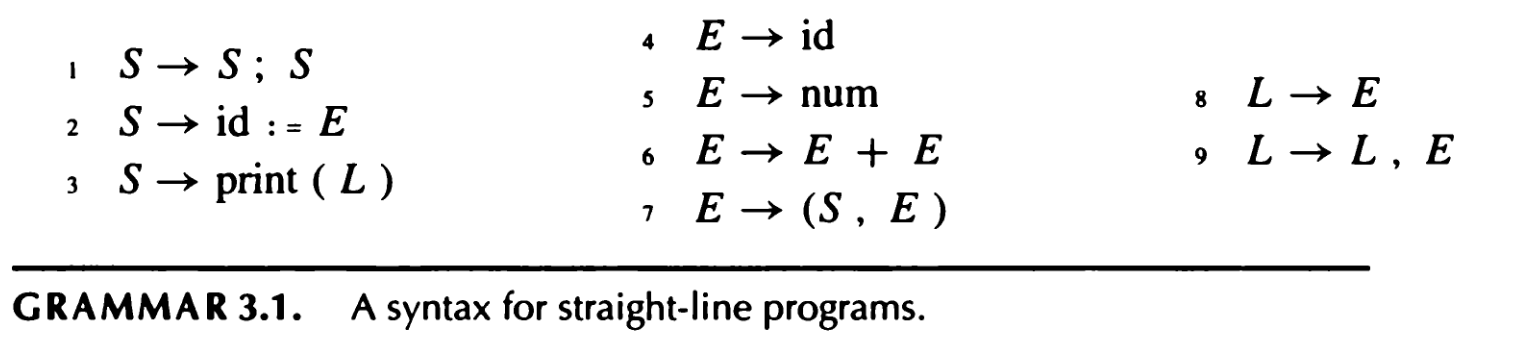
\includegraphics[width=0.5\textwidth,height=0.5\textheight,keepaspectratio]{slbg}

As before, we say that a language is a set of strings; each string is a finite
sequence of symbols taken from a finite alphabet. For parsing, the strings are
source programs, the symbols are lexical tokens, and the alphabet is the set
of token types returned by the lexical analyzer.

A leftmost
derivation is one in which the leftmost nonterminal symbol is always the one
expanded; in a rightmost derivation, the rightmost nonterminal is always next
to be expanded.

A parse tree is made by connecting each symbol in a derivation to the one
from which it was derived, as shown in Figure 3.3. Two different derivations
can have the same parse tree.

A grammar is ambiguous if it can derive a sentence with two different parse
trees.

Parsers must read not only terminal symbols such as +, -, num, and so on, but
also the end-of-file marker. We will use \$ to represent end of file.

Suppose S is the start symbol of a grammar. To indicate that \$ must come
after a complete S-phrase, we augment the grammar with a new start symbol
S' and a new production S' $\rightarrow$ S\$.

\textbf{Predictive Parsing:} Some grammars are easy to parse using a simple algorithm known as 
recursive descent. Predictive parsing works only on grammars where
the first terminal symbol of each subexpression provides enough information
to choose which production to use.

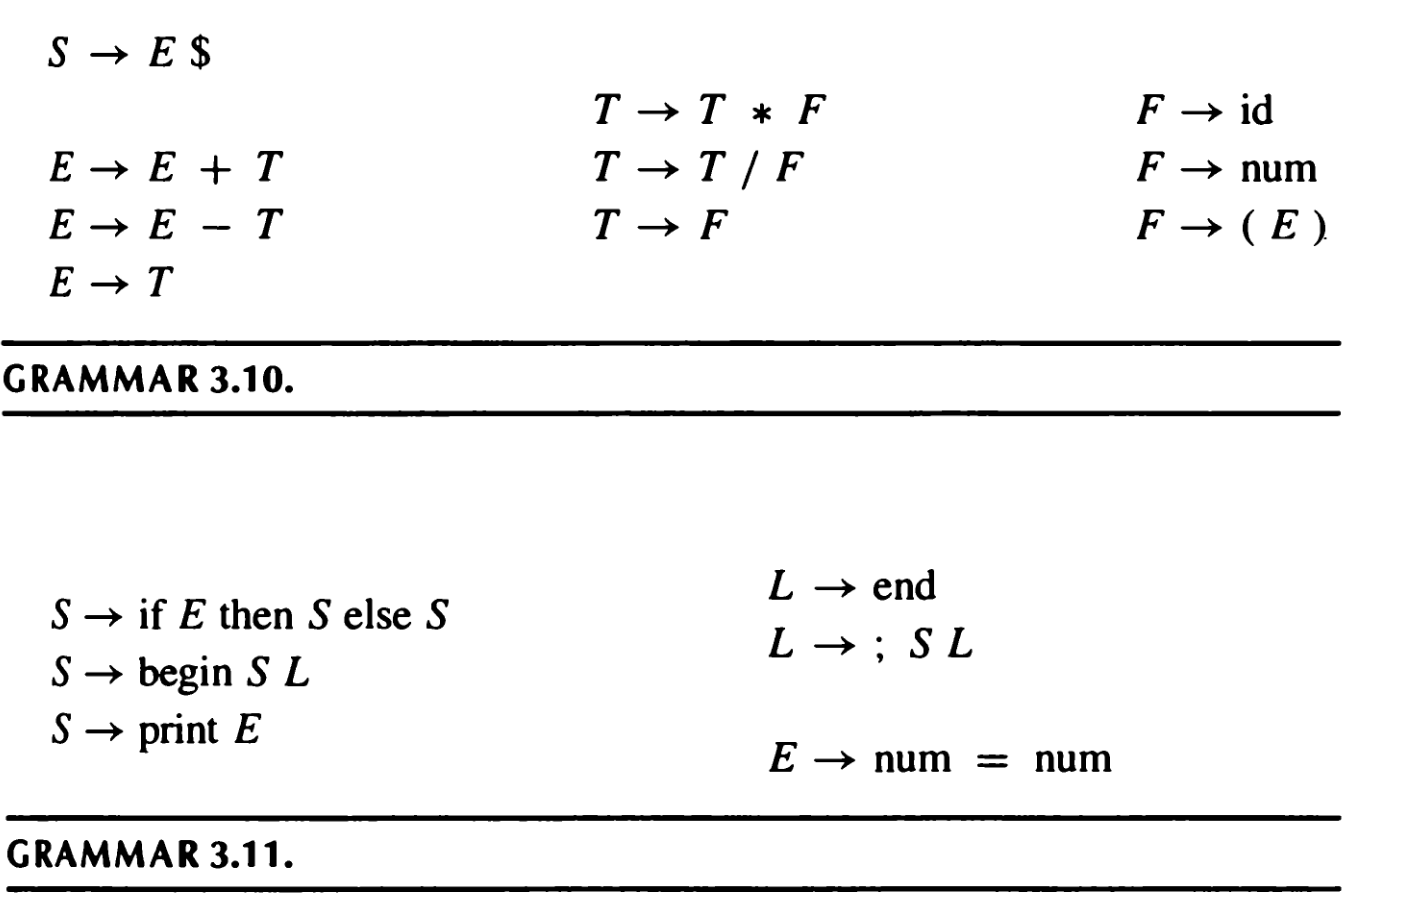
\includegraphics[width=0.5\textwidth,height=0.5\textheight,keepaspectratio]{pp}

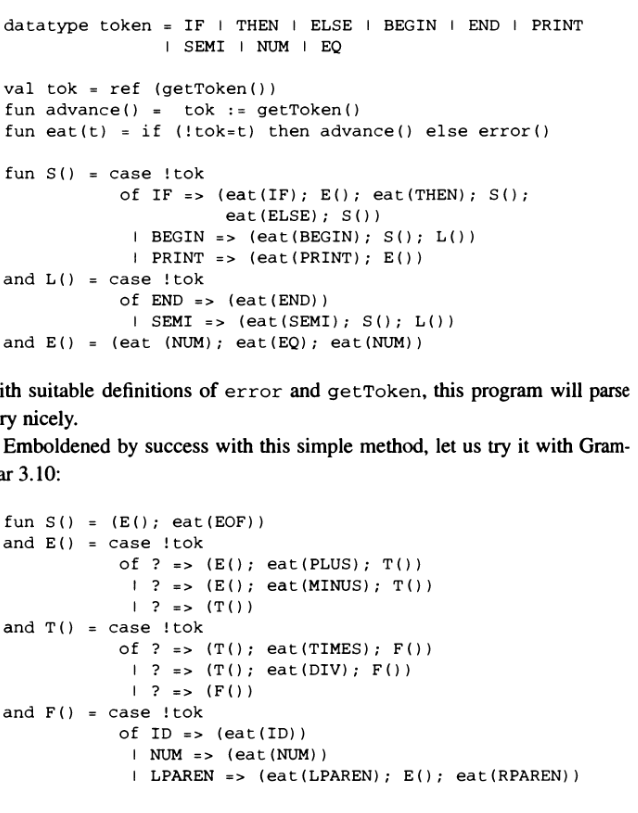
\includegraphics[width=0.5\textwidth,height=0.5\textheight,keepaspectratio]{pp2}

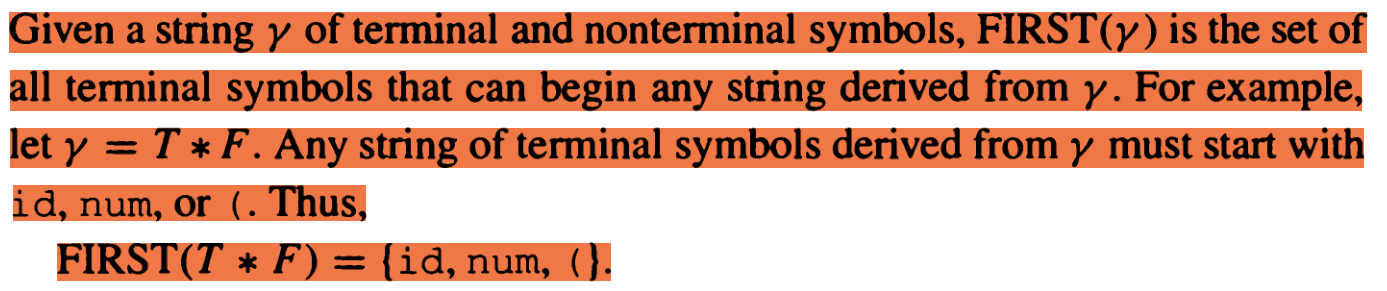
\includegraphics[width=0.5\textwidth,height=0.5\textheight,keepaspectratio]{first}

If two different productions $X \rightarrow \gamma_1 and X \rightarrow \gamma_2$ have the same left-
hand-side symbol $(X)$ and their right-hand sides have overlapping FIRST
sets, then the grammar cannot be parsed using predictive parsing.

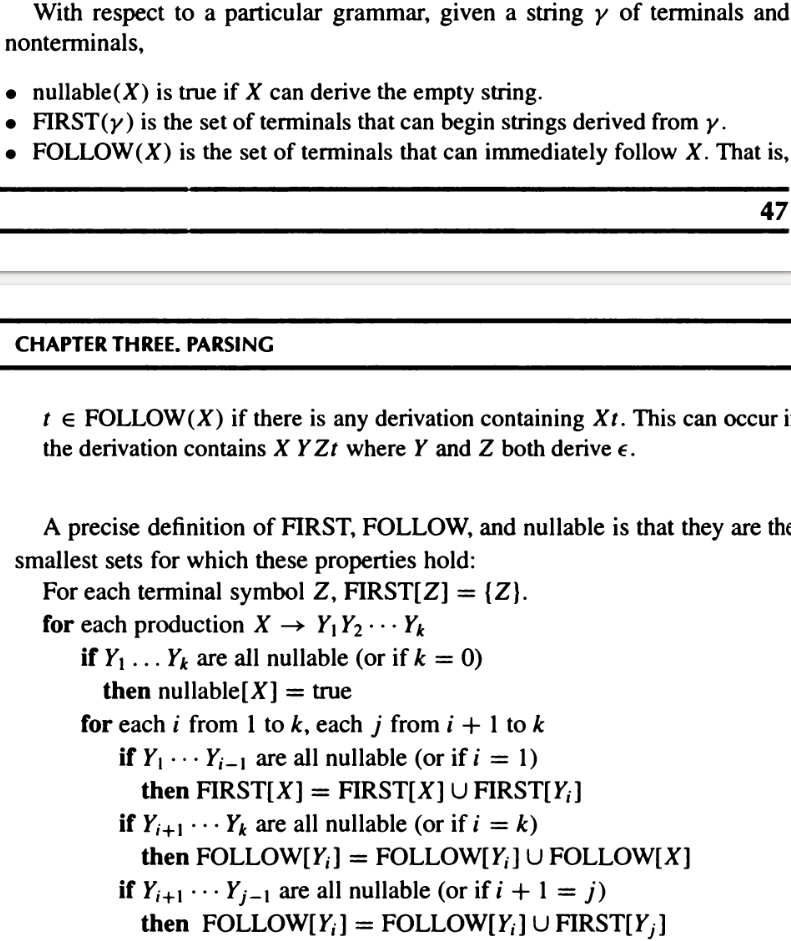
\includegraphics[width=0.5\textwidth,height=0.5\textheight,keepaspectratio]{follow}

The set of sym-
bols is the union of the non-terminal and terminal sets. 

Each production
has a semantic action associated with it.  A production with a semantic action is called a
rule.  Parsers perform bottom-up, left-to-right evaluations of parse trees using semantic
actions to compute values as they do so
Given a production $P = A \rightarrow \alpha$
, the corre-
sponding semantic action is used to compute a value for $A$
from the values of the symbols
in $\alpha$.  If
$A$
has no value, the semantic action is still evaluated but the value is ignored.
Each  parse  returns  the  value  associated  with  the  start  symbol
$S$
of  the  grammar. $A$
parse returns a nullary value if the start symbol does not carry a value.

An ML-Yacc specification consists of three parts, each of which is separated from the
others by a \%\% delimiter.  The general format is:
ML-Yacc user declarations
\%\%
ML-Yacc declarations
\%\%
ML-Yacc rules
Comments have the same lexical definition as they do in Standard ML and can be
placed in any ML-Yacc section

After the first \%\%, the following words and symbols are reserved:
\begin{minted}{cpp}
of for = { } , * -> :  | ( )
\end{minted}
% The following classes of ML symbols are used:
% dentifiers:
% non-symbolic ML identifiers, which consist of an alphabetic character fol-
% lowed  by  one  or  more  alphabetic  characters,  numeric  characters,  primes “
% ’
% ”,  or
% underscores “
% _
% ”.
% type variables:
% non-symbolic ML identifier starting with a prime “
% ’
% ”
% integers:
% one or more decimal digits.
% qualified identifiers:
% an identifier followed by a period.
% The following classes of non-ML symbols are used:
% % identifiers:
% a percent sign followed by one or more lowercase alphabet letters.  The
% valid % identifiers are:
% %arg %eop %header %keyword %left %name %nodefault %nonassoc
% %nonterm %noshift %pos %prec %prefer %pure %right %start
% %subst %term %value %verbose

code:
This  class  is  meant  to  hold  ML  code.   The  ML  code  is  not  parsed  for  syntax
errors.  It consists of a left parenthesis followed by all characters up to a balancing
right parenthesis.  Parentheses in ML comments and ML strings are excluded from
the count of balancing parentheses.

In ML-YACC user declarations section you can define values available in the semantic actions of the rules in the user declarations  section.   It  is  recommended  that  you  keep  the  size  of  this  section  as  small  as
possible and place large blocks of code in other modules.

The  ML-Yacc  declarations  section  is  used  to  make  a  set  of  required  declarations  and
a set of optional declarations.  

You must declare the type of basic payload position values using the
\%pos
declaration.
The syntax is
\%pos
ML-type
. This type MUST be the same type as that which is actually
found in the lexer.  It cannot be polymorphic.
You may declare whether the parser generator should create a verbose description of the parser in a “.desc” file. This  is  useful  for  debugging  your  parser  and  for  finding  the
causes of shift/reduce errors and other parsing conflicts.

You may also declare whether the semantic actions are free of significant side-effects
and  always  terminate.   Normally,  ML-Yacc  delays  the  evaluation  of  semantic  actions
until the completion of a successful parse.  This ensures that there will be no semantic
actions to “undo” if a syntactic error-correction invalidates some semantic actions.  If,
however, the semantic actions are free of significant side-effects and always terminate,
the results of semantic actions that are invalidated by a syntactic error-correction can
always be safely ignored.

Parsers run faster and need less memory when it is not necessary to delay the eval-
uation of semantic actions.  You are encouraged to write semantic actions that are free
of side-effects and always terminate and to declare this information to ML-Yacc.

A semantic action is free of significant side-effects if it can be re-executed a reasonably
small number of times without affecting the result of a parse.  (The re-execution occurs
when the error-correcting parser is testing possible corrections to fix a syntax error, and
the number of times re-execution occurs is roughly bounded, for each syntax error, by the
number of terminals times the amount of lookahead permitted for the error-correcting
parser).

You must specify the name of the parser with command
\%name
name
.  If you decide to
call your parser “
\ita{My}
Parser
” then you will need the declaration:
87
\%name My
This declaration must agree with the ML-Lex command
\%header


You  must  define  the  terminal  and  non-terminal  sets  using  the
\%term
and
\%nonterm
declarations, respectively.  These declarations are like an ML datatype definition.
The types cannot be polymorphic. Do not use any locally defined types from the user
declarations section of the specification

Terminals are written in Capitals whereas non terminals are written in small.

Consider 

\%nonterm elabel of (symbol * exp)

Here since the supplemented payload is a tuple, parenthesis is required.

You may want each invocation of the entire parser to be parameterised by a particular
argument, such as the file name of the input being parsed in an invocation of the parser.
The
\%arg
declaration  allows  you  to  specify  such  an  argument.   (This  is  often  cleaner
than using “global” reference variables.)  The declaration
\%arg
Any-ML-pattern
:
ML-type
specifies  the  argument  to  the  parser,  as  well  as  its  type.   If
\%arg
is  not  specified,  it
defaults to
() :  unit
.
Note that ML-Lex also has a
\%arg
directive, but the two are independent and may
have different types.
For example:

107
\%arg (fileName) : string


You  should  specify the  set  of terminals  that  may  follow  the  start symbol,  also  called
end-of-parse symbols, using the
\%eop
declaration.  The
\%eop
keyword should be followed
by the list of terminals.  This is useful, for example, in an interactive system where you
want to force the evaluation of a statement before an end-of-file (remember,  a parser
delays the execution of semantic actions until a parse is successful).
ML-Yacc has no concept of an end-of-file.  You must define an end-of-file terminal
(
EOF
, perhaps) in the
\%term
declaration.  You must declare terminals which cannot be
shifted, such as end-of-file, in the
\%noshift
declaration.  The
\%noshift
keyword should
be followed by the list of non-shiftable terminals.  An error message will be printed if a
non-shiftable terminal is found on the right hand side of any rule, but ML-Yacc will not
prevent you from using such grammars.


You should list the precedence declarations in order of increasing (tighter-binding) prece-
dence.   Each  precedence  declaration  consists  of  a
\%
keyword  specifying  associativity
followed by a list of terminals.  You may place more than one terminal at a given prece-
dence level,  but you cannot specify non-terminals.  The keywords are
\%left
,
\%right
,
and
\%nonassoc
, standing for their respective associativities.

The
\%nodefault
declaration  suppresses  the  generation  of  default  reductions

Include the
\%pure
declaration if the semantic actions are free of significant side effects
and always terminate.  It is suggested that you begin developing your language without
this directive

You  may  define  the  start  symbol  using  the
\%start
declaration.   Otherwise  the  non-
terminal for the first rule will be used as the start non-terminal.
The keyword
\%start
should be followed by the name of the starting non-terminal.  This non-terminal should
not be used on the right hand side of any rules, to avoid conflicts between reducing to
the start symbol and shifting a terminal.

Include the
\%verbose
declaration to produce a verbose description of the LALR parser.
The name of this file is the name of the specification file with a “
.desc
” appended to it,
for example
pi.yacc.desc
.
This file is helpful for debugging, and has the following format:

1.  A summary of errors found while generating the LALR tables.

2.  A detailed description of all errors.

3.  A description of the states of the parser. Each state is preceded by a list of conflicts
in the state.

Specify all keywords in your grammar here.  The
\%keyword
should be followed by a list
of terminal names

List terminals to prefer for insertion after the command
\%prefer
.  Corrections which
insert a terminal on this list will be chosen over other corrections, all other things being
equal.

The error-correction algorithm may also insert terminals with values.  You must supply
a value for such a terminal.  The keyword should be followed by a terminal and a piece
of code (enclosed in parentheses) that when evaluated supplies the value.  There must
be a separate
\%value
declaration for each terminal with a value that you wish may be
inserted or substituted in an error correction.  The code for the value is not evaluated
until the parse is successful.

\textbf{ML-YACC Rules}

The rules section contains the context-free grammar productions and their associated
semantic actions.
A rule consists
of a left hand side non-terminal, followed by a colon, followed by a list of right hand side
clauses. The right hand side clauses should be separated by bars.
Each clause consists of
a list of non-terminal and terminal symbols, followed by an optional
\%prec
declaration,
and then followed by the code to be evaluated when the rule is reduced.
The  optional
\%prec
consists  of  the  keyword
\%prec
followed by  a  terminal  whose
precedence should be used as the precedence of the rule.
The values of those symbols in a right hand side clause which have values are available
inside the code

\begin{minted}{SML}
    141   path: IDE   ((Name (IDE,fileName,IDEleft,IDEright)
\end{minted}
Each  position  value  has  the  general  form
\{
symbol  name
\}\{
n+1
\}
,  where
\{
n
\}
is  the
number of occurrences of the symbol to the left of the symbol.  If the symbol occurs
only once in the rule,
\{
symbol name
\}
may also be used.  For example, if in rule “
path
”
above, there had been two
IDE
’s in the list of symbols, we could have referred to their
values as
IDE1
and
IDE2
.

Positions for all the symbols are also available.  The payload positions are given by
\{
symbol  name
\}\{
n+1
\}
left
and
\{
symbol  name
\}\{
n+1
\}
right
.   where
\{
n
\}
is  defined  as
before.  For example we see the use of
IDEleft
and
IDEright
on line 141.
If in rule “
path
” above,  there had been two
IDE
’s in the list of symbols,  we could
have referred to their left and right positions as
IDE1left
,
IDE1right
,
IDE2left
and
IDE2right
.

The position for a null right-hand-side of a production is assumed to be the leftmost
position of the lookahead terminal which is causing the reduction.  This position value
is available in
defaultPos

The  value  to  which  the  code  evaluates  is  used  as  the  value  of  the  non-terminal.
The type of the value and the non-terminal must match.  The value is ignored if the
non-terminal has no value, but is still evaluated for side-effects.

\begin{minted}{SML}
142 datatype Life = Life of Year * Year      * int * int
143 and Year = Year of int * int * int  * int * int
\end{minted}
The two integers at the end of each of lines 142 and 143 give the position of the con-
structions in the source file.  They will be needed for error messages.
The tokens representing years, months and days will have a supplemental payload
of one integer; they are declared in the ML-Yacc declarations section of the file
my.yacc
as:
\begin{minted}{SML}
144 %term YMD of int
\end{minted}
This means that the tokens
YMD
generated by the lexer will have a payload of type
int
* int * int
.  The lexer rules in file
my.lex
might be
\begin{minted}{SML}
145 {int} => (T.YMD(stoi yytext,!line,!col))
\end{minted}
where function
stoi :  string -> int
converts a string of digits to the corresponding
integer.
Parser rules in file
my.yacc
will pull these three integers together to form the two
years and the life:
\begin{minted}{SML}
146 life: year HYPHEN year
147 ((Life (year1,year2,year1left,year1right)))
148 year: YMD COLON YMD COLON YMD
149 ((Year (YMD1,YMD2,YMD3,YMD1left,YMD1right)
\end{minted}


Add
\%prec
declarations to the rules to say which terminal’s precedence and as-
sociativity  are  to  be  used  with  which  rules

The language specified by this project requires that function application be left
associative  as  in  ML, i.e.
f g 2
means
(f g) 2
.   Now  function  application  is  a
non-terminal,
fun\_appl
, in the ML-Yacc specification, and non-terminals cannot
be placed in the
\%left
,
\%right
and
\%nonassoc
declarations — what can we do?
The solution is to create a new terminal,
FUN\_APPL
, by declaring it in the
\%term
declaration,  and then defining the required precedence and associativity on line
\begin{minted}{SML}
170.  The corresponding rule becomes:
175 fun_appl:   (* Function application has precedence
176 and associativity defined by dummy
177 terminal FUN_APPL. *)
178 name e     %prec FUN_APPL  ((name,e))
\end{minted}

\textbf{Error recovery in predictive parsing (LL (1)):}

\iph{0.5}{erpp}

\subsection{LR(0)}

\iph{0.5}{lr0}

Note: 'X' in Goto can be either a terminal or non terminal
 
\iph{0.5}{lr01}

\iph{0.5}{lr02}

\subsection{SLR}

\iph{0.5}{slr}

\ph{slr2}

\subsection{LR(1)}

\ph{lr1}

\ph{lr2}

\ph{hier}

\ph{yaccpref}

\ph{yaccpref2}

\ph{yaccpref3}

\ph{yaccpref4}

\ph{yaccpref5}

Popping states from the stack can lead to seemingly "im

\ph{err}

\ph{gerr}

Read page 79, 80, 81 from text.

\section{AST}
However, an LR parser does perform reductions, and associated semantic
actions, in a deterministic and predictable order: a bottom-up, left-to-right
traversal of the parse tree. In other words, the (virtual) parse tree is traversed
in postorder.

It is possible to write an entire compiler that fits within the semantic action
phrases of an ML-Yacc parser. However, such a compiler is difficult to read
and maintain. And this approach constrains the compiler to analyze the 
program in exactly the order it is parsed.

Technically, a parse tree has exactly one leaf for each token of the input and one internal node for each
grammar rule reduced during the parse.
Such a parse tree, which we will call a concrete parse tree representing the
concrete syntax of the source language, is inconvenient to use directly. Many
of the punctuation tokens are redundant and convey no information - they are
useful in the input string, but once the parse tree is built, the structure of the
tree conveys the structuring information more conveniently.
Furthermore, the structure of the parse tree depends too much on the 
grammar! The grammar transformations shown in Chapter 3 - factoring, 
elimination of left recursion, elimination of ambiguity - involve the introduction of
extra nonterminal symbols and extra grammar productions for technical 
purposes. These details should be confined to the parsing phase and should not
clutter the semantic analysis.

An abstract syntax makes a clean interface between the parser and the
later phases of a compiler (or, in fact, for the later phases of other kinds of
program-analysis tools such as dependency analyzers). The abstract syntax
tree conveys the phrase structure of the source program, with all parsing 
issues resolved but without any semantic interpretation.

So the parser uses the 
concrete syntax to build a parse tree for the abstract syntax.
The semantic analysis phase takes this abstract syntax tree; it is not bothered by
the ambiguity of the grammar, since it already has the parse tree!

The lexer must pass the source-file positions of the beginning and end of
each token to the parser. The ML-Yacc parser makes these positions available
(in the semantic action fragments): for each terminal or nonterminal such as
FOO or FOOl on the right-hand side of a rule, the ML variable FOOlef t or
FOOllef t stands for the left-end position of the terminal or nonterminal, and
FOOright or FOOl right stands for the right-end position.

The Tiger language treats adjacent function declarations as (possibly) 
mutually recursive. The FunctionDec constructor of the abstract syntax takes
a list of function declarations, not just a single function. The intent is that
this list is a maximal consecutive sequence of function declarations. Thus,
functions declared by the same FunctionDec can be mutually recursive.

The TypeDec constructor also takes a list of type declarations, for the
same reason;

There is no abstract syntax for "\&" and "$\vert$" expressions; instead, $e_1\&e_2$ is
translated as if $e_1$ then $e_2$ else 0, and $e_1 \vert e_2$ is translated as though it had
been written if $e_1 then 1 else e_2$
Similarly, unary negation (-x) should be represented as subtraction (0 -
x) in the abstract syntax. Also, where the body of a Let Exp has multiple
statements, we must use a SeqExp. An empty statement is represented by
SeqExp[].

The semantic analysis phase of the compiler will need to keep track of
which local variables are used from within nested functions. The escape
component of a VarDec, ForExp, or formal parameter is used to keep track
of this. The parser should leave each escape set to true, which is a 
conservative approximation. The field type is used for both formal parameters
and record fields; escape has meaning for formal parameters, but for record
fields it can be ignored.
Having the escape fields in the abstract syntax is a "hack," since 
escaping is a global, nonsyntactic property. But leaving escape out of the Absyn
would require another data structure for describing escapes.
\section{Semantic Analysis}
This phase is characterized by the maintenance of symbol tables (also called
environments) mapping identifiers to their types and locations.

\ph{sem1}

\ph{sem2}

\ph{sem3}

\ph{sem4}


\section{Activation Records}
For the remainder of this chapter we will consider languages with stackable
local variables and postpone discussion of higher-order functions to 
Chapter 15.

\ph{r1}

\ph{r2}

\ph{r3}

\ph{r4}

\ph{r5}

\ph{r6}

\ph{r7}

\ph{r8}

Figure 6.2 shows a typical stack frame layout. The frame has a set of 
incoming arguments (technically these are part of the previous frame but they
are at a known offset from the frame pointer) passed by the caller. The 
return address is created by the CALL instruction and tells where (within the
calling function) control should return upon completion of the current 
function. Some local variables are in this frame; other local variables are kept in
machine registers. Sometimes a local variable kept in a register needs to be
saved into the frame to make room for other uses of the register; there is an
area in the frame for this purpose. Finally, when the current function calls
other functions, it can use the outgoing argument space to pass parameters.

Suppose a function g(...) calls the function f($a_1, \dots , a_n$). We say g is the
caller and f is the callee.
On entry to f, the stack pointer points to the first
argument that g passes to f. On entry, f allocates a frame by simply 
subtracting the frame size from the stack pointer SP. The old SP becomes the current frame pointer FP.

FP is a
"fictional" register whose value is always SP+framesize.
Why talk about a frame pointer at all? Why not just refer to all variables,
parameters, etc. by their offset from SP, if the frame size is constant? The
frame size is not known until quite late in the compilation process, when the
number of memory-resident temporaries and saved registers is determined.

Suppose a function f is using register r to hold a local variable and calls procedure g, which also uses r for
its own calculations. Then r must be saved (stored into a stack frame) before
g uses it and restored (fetched back from the frame) after g is finished using
it. But is it f's responsibility to save and restore the register, or g's? We say
that r is a caller-save register if the caller (in this case, f) must save and 
restore the register, and r is callee-save if it is the responsibility of the callee
(in this case, g).

therefore the
first k arguments (for k = 4 or k = 6, typically) of a function are passed in
registers $r_p, \dots, r_{p+k - 1}$ and the rest of the arguments are passed in memory.

\ph{r9}

\ph{r10}

\ph{r11}

To resolve the contradiction that
parameters are passed in registers, but have addresses too, the first k 
parameters are passed in registers; but any parameter whose address is taken must
be written to a memory location on entry to the function. To satisfy printf,
the memory locations into which register arguments are written must all be
consecutive with the memory locations in which arguments k + 1, k + 2, etc.
are written. Therefore, C programs can't have some of the arguments saved
in one place and some saved in another - they must all be saved contiguously.

When function g calls function f, eventually f must return. It needs to know
where to go back to. If the call instruction within g is at address a, then
(usually) the right place to return to is a + 1, the next instruction in g. This is
called the return address.

On modern machines, the call instruction merely puts the return address
(the address of the instruction after the call) in a designated register. A non-
leaf procedure will then have to write it to the stack (unless interprocedural
register allocation is used), but a leaf procedure will not.

Many of the local variables will be allocated to registers, as will the
intermediate results of expression evaluation. Values are written to memory
(in the stack frame) only when necessary for one of these reasons:

\ph{r12}

We will say that a variable escapes if it is passed by reference, its address
is taken (using C's \& operator), or it is accessed from a nested function.

Unfortunately, the conditions in our list don't manifest
themselves early enough. When the compiler first encounters the declaration
of a variable, it doesn't yet know whether the variable will ever be passed
by reference, accessed in a nested procedure, or have its address taken; and
doesn't know how many registers the calculation of expressions will require
An industrial-strength compiler must assign provisional locations
to all formals and locals, and decide later which of them should really go in registers.

In languages that allow nested function declarations, the inner functions may use variables declared in outer functions. This
language feature is called block structure.

There are several methods to allow inner functions to access outer ones:

\ph{r13}

I will describe in detail only the method of static links.

\ph{arpb}

\ph{r14}

\ph{r15}

The type frame holds information about formal parameters and local 
variables allocated in this frame. To make a new frame for a function f with k
formal parameters, call newFrame \{name=f formals=l\}, where l is a list
of k booleans: true for each parameter that escapes and false for each
parameter that does not. The result will be a frame object.

The access type describes formals and locals that may be in the frame or
in registers.

\ph{r16}

The Frame. formals interface function extracts a list of it "accesses" 
denoting the locations where the formal parameters will be kept at run time, as
seen from inside the callee. Parameters may be seen differently by the caller.
For example, if parameters are passed on the stack, the caller
may put a parameter at offset 4 from the stack pointer, but the callee sees it at
offset 4 from the frame pointer. Or the caller may put a parameter into register
6, but the callee may want to move it out of the way and always access it from register 13.

because of this "shift of view" newFrame must calculate two things:
• How the parameter will be seen from inside the function (in a register, or in a
frame location);
• What instructions must be produced to implement the "view shift."

Some local variables are kept in the frame; others are kept in registers. To
allocate a new local variable in a frame f, the semantic analysis phase calls
Frame.allocLocal(f)(true). This returns an InFrame access with an offset from the frame pointer.
The boolean argument to allocLocal specifies whether the new 
variable escapes and needs to go in the frame; if it is false, then the variable
can be allocated in a register. Thus, allocLocal (f) ( false) might create
InReg($t_{481}$).

We use the word
temporary to mean a value that is temporarily held in a register, and the word
label to mean some machine-language location whose exact address is yet to be determined.
\section{Translation To Intermediate Code}
The front end of the compiler does lexical analysis, parsing,
semantic analysis, and translation to intermediate representation. The back
end does optimization of the intermediate representation and translation to
machine language.

\ph{ir1}

For our compiler the intermediate representation tree language is defined by the signature tree, as shown in figure

\ph{ir2}

Meaning:

expressions (exp), which stand for the computation of some value (possibly
with side effects):

\ph{ir3}

\ph{ir4}

\ph{ir5}

What should the representation of an abstract syntax expression Absyn.exp
be in the Tree language? At first it seems obvious that it should be Tree.exp.
However, this is true only for certain kinds of expressions, the ones that 
compute a value. Expressions that return no value (such as some procedure calls,
or while expressions in the Tiger language) are more naturally represented
by Tree.stm. And expressions with Boolean values, such as $a > b$, might
best be represented as a conditional jump - a combination of Tree.stm and
a pair of destinations represented by Temp. labels.
Therefore, we will make a datatype exp in the Translate module to
model these three kinds of expressions:

\ph{ir6}

Sometimes we will have an expression of one kind and we will need to
convert it to an equivalent expression of another kind. For example, the Tiger
statement

flag := $(a>b \vert c<d)$

\ph{ir7}

\ph{ir8}

\ph{ir9}

\section{Basic Blocks And Traces}
It's useful to be able to evaluate the subexpressions of an 
expression in any order. If tree expressions did not contain ESEQ and CALL nodes,
then the order of evaluation would not matter.

\ph{81}

We can take any tree and rewrite it into an equivalent tree without any of
the cases listed above. Without these cases, the only possible parent of a SEQ
node is another SEQ; all the SEQ nodes will be clustered at the top of the tree.
This makes the SEQs entirely uninteresting; we might as well get rid of them
and make a linear list of Tree.stms.

The transformation is done in three stages: First, a tree is rewritten into a
list of canonical trees without SEQ or ESEQ nodes; then this list is grouped
into a set of basic blocks, which contain no internal jumps or labels; then
the basic blocks are ordered into a set of traces in which every CJUMP is
immediately followed by its false label.

\ph{82}

How can the ESEQ nodes be eliminated? The idea is to lift them higher and
higher in the tree, until they can become SEQ nodes.

\ph{83}

\ph{84}

\ph{85}

\ph{86}

\ph{87}

\ph{88}

\ph{89}

\ph{811}

\ph{812}

\ph{813}

\ph{814}

\ph{815}

\ph{816}

We will apply this algorithm to each function-body in turn. The procedure
"epilogue" (which pops the stack and returns to the caller) will not be part of
this body, but is intended to follow the last statement. When the flow of 
program execution reaches the end of the last block, the epilogue should follow.
But it is inconvenient to have a "special" block that must come last and that
has no JUMP at the end. Thus, we will invent a new label done - intended
to mean the beginning of the epilogue - and put a JUMP(NAME done) at the
end of the last block.

Now the basic blocks can be arranged in any order, and the result of executing
the program will be the same - every block ends with a jump to the 
appropriate place. We can take advantage of this to choose an ordering of the blocks
satisfying the condition that each CJUMP is followed by its false label.

At the same time, we can also arrange that many of the unconditional
jumps are immediately followed by their target label. This will allow the
deletion of these jumps, which will make the compiled program run a bit
faster.

\ph{818}

\ph{819}

\ph{820}


\end{document}
